\documentclass[compress]{beamer}
\usepackage{irbookslide}
\usepackage{irilmenau2}
\usepackage{tikz}
\usepackage{url}
\usepackage{ifxetex}
%\RequireXeTeX
\usepackage{fontspec} % zahteva paket euenc
\usepackage{xunicode}
\usepackage{xltxtra}
\usepackage{polyglossia}
\usepackage{minted}
\usepackage[noend]{algorithmic}
\renewcommand{\algorithmicrequire}{\textbf{Input:}}
\renewcommand{\algorithmicensure}{\textbf{Output:}}
\renewcommand{\algorithmiccomment}[1]{\hfill \{\myred{#1}\}}
\usepackage{xcolor,colortbl}
\usepackage{textcomp}
\usepackage{unicode-math}
%\usepackage{hyphenat}
%\setdefaultlanguage[script=Latin]{serbian}

\title{Grafovi}
\author{\textcopyright \ \ Goodrich, Tamassia, Goldwasser}
\institute{Katedra za informatiku, Fakultet tehničkih nauka, Univerzitet u
Novom Sadu}
\date{2014.}
\subject{Predavanja sa ASP}

\begin{document}

\frame{\titlepage}

\section[Pojam]{Pojam grafa}

\begin{frame}[fragile]
  \frametitle{Pojam grafa}
  \begin{itemize}
    \item \myred{graf} je par $(V,E)$
    \begin{itemize}
      \item $V$ je set čvorova (\textit{vertices})
      \item $E$ je skup grana (\textit{edges})
      \item ćvorovi i grane čuvaju elemente
    \end{itemize}
    \item primer:
    \begin{itemize}
      \item čvorovi predstavljaju aerodrome i čuvaju šifre aerodroma
      \item grane predstavljaju letove između aerodroma i čuvaju dužinu puta
    \end{itemize}
  \end{itemize}
  \begin{center}
    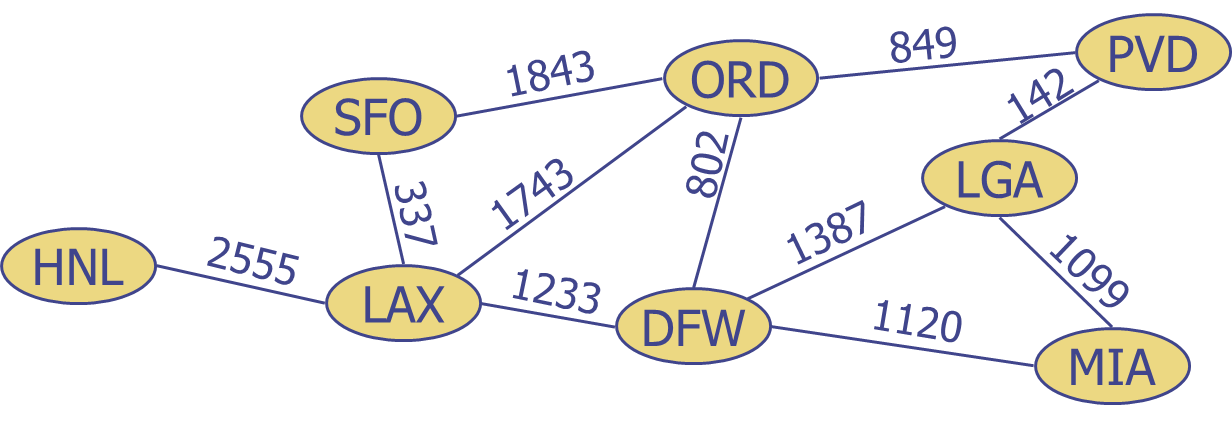
\includegraphics[width=10.5cm]{asp-14-pic01.png}
  \end{center}
\end{frame}

\begin{frame}[fragile]
  \frametitle{Vrste grana}
  \begin{columns}
    \begin{column}[t]{8cm}
      \begin{itemize}
        \item usmerena grana
        \begin{itemize}
          \item uređeni par čvorova $(u,v)$
          \item prvi čvor $u$ je polazište
          \item drugi čvor $v$ je odredište
          \item npr. konkretan let aviona
        \end{itemize}
        \item neusmerena grana
        \begin{itemize}
          \item neuređeni par čvorova $(u,v)$
          \item npr. putanja leta
        \end{itemize}
        \item usmereni graf
        \begin{itemize}
          \item sve grane su usmerene
          \item npr. mreža letova
        \end{itemize}
        \item neusmereni graf
        \begin{itemize}
          \item sve grane su neusmerene
          \item npr. mreža putanja
        \end{itemize}
      \end{itemize}
    \end{column}
    \begin{column}[t]{4cm}
      \begin{center}
        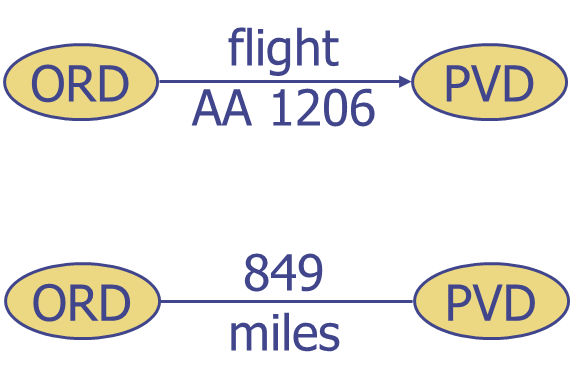
\includegraphics[width=4cm]{asp-14-pic02.png}
      \end{center}
    \end{column}
  \end{columns}
\end{frame}

\begin{frame}[fragile]
  \frametitle{Primene}
  \begin{columns}
    \begin{column}[t]{6cm}
      \begin{itemize}
        \item elektronska kola
        \begin{itemize}
          \item štampane ploče
          \item integrisana kola
        \end{itemize}
        \item transportne mreže
        \begin{itemize}
          \item putevi
          \item avionski letovi
        \end{itemize}
        \item računarske mreže
        \begin{itemize}
          \item lokalne mreže
          \item Internet
        \end{itemize}
        \item baze podataka
        \begin{itemize}
          \item ER dijagrami
        \end{itemize}
      \end{itemize}
    \end{column}
    \begin{column}[t]{6cm}
      \begin{center}
        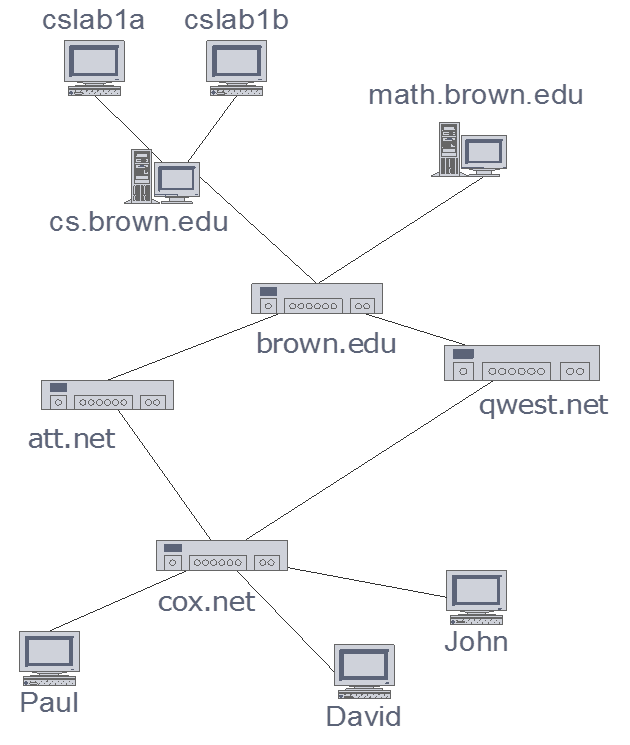
\includegraphics[width=6cm]{asp-14-pic03.png}
      \end{center}
    \end{column}
  \end{columns}
\end{frame}

\begin{frame}[fragile]
  \frametitle{Terminologija $_{1}$}
  \begin{columns}
    \begin{column}[t]{6cm}
      \begin{itemize}
        \item krajevi grane
        \begin{itemize}
          \item $U$ i $V$ su krajevi $a$
        \end{itemize}
        \item grane incidentne na čvoru
        \begin{itemize}
          \item $a$, $d$ i $b$ su incidentni na $V$
        \end{itemize}
        \item susedni čvorovi
        \begin{itemize}
          \item povezani granom
          \item $U$ i $V$ su susedni
        \end{itemize}
        \item stepen čvora
        \begin{itemize}
          \item broj grana kojima je on kraj
          \item stepen of $X$ je 5
        \end{itemize}
        \item paralelne grane: $h$ i $i$
        \item petlja: $j$
      \end{itemize}
    \end{column}
    \begin{column}[t]{6cm}
      \begin{center}
        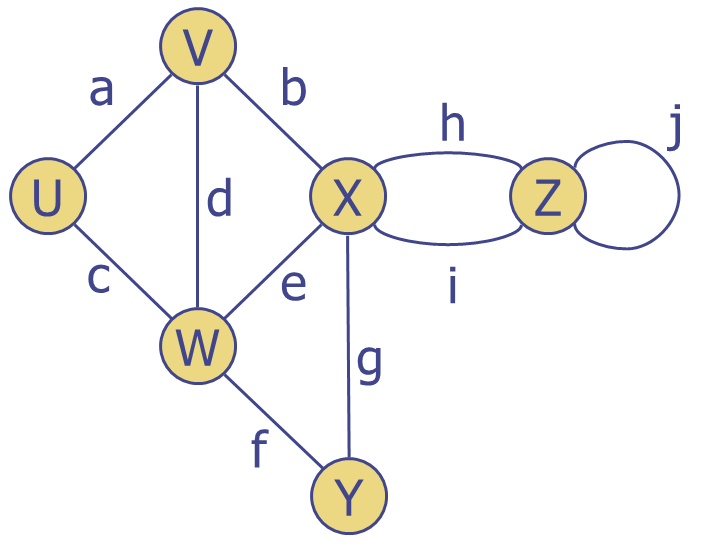
\includegraphics[width=6cm]{asp-14-pic04.png}
      \end{center}
    \end{column}
  \end{columns}
\end{frame}

\begin{frame}[fragile]
  \frametitle{Terminologija $_{2}$}
  \begin{columns}
    \begin{column}[t]{7.5cm}
      \begin{itemize}
        \item putanja
        \begin{itemize}
          \item sekvenca naizmenično čvorova i grana
          \item počinje sa čvorom
          \item završava sa čvorom
          \item svakoj grani prethodi i sledi njen kraj
        \end{itemize}
        \item prosta putanja
        \begin{itemize}
          \item svi čvorovi i grane su različiti
        \end{itemize}
        \item primeri
        \begin{itemize}
          \item $P_{1}=(V,b,X,h,Z)$ je prosta
          \item $P_{2}=(U,c,W,e,X,g,Y,f,W,d,V)$ nije prosta
        \end{itemize}
      \end{itemize}
    \end{column}
    \begin{column}[t]{4.5cm}
      \begin{center}
        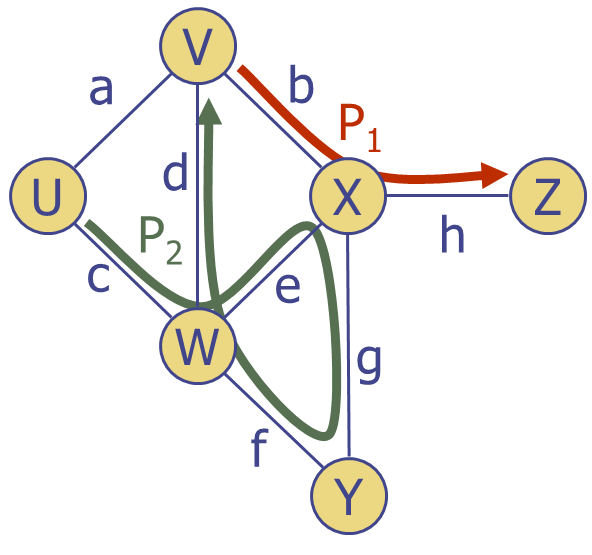
\includegraphics[width=4.5cm]{asp-14-pic05.png}
      \end{center}
    \end{column}
  \end{columns}
\end{frame}

\begin{frame}[fragile]
  \frametitle{Terminologija $_{3}$}
  \begin{columns}
    \begin{column}[t]{7.5cm}
      \begin{itemize}
        \item petlja
        \begin{itemize}
          \item cirkularna sekvenca naizmenično čvorova i grana
          \item svakoj grani prethodi i sledi njen kraj
        \end{itemize}
        \item prosta petlja
        \begin{itemize}
          \item s vi čvorovi i grane su različiti
        \end{itemize}
        \item primeri
        \begin{itemize}
          \item $C_{1}=(V,b,X,g,Y,f,W,c,U,a,V)$ je prosta
          \item $C_{2}=(U,c,W,e,X,g,Y,f,W,d,V,a,U)$ nije prosta
        \end{itemize}
      \end{itemize}
    \end{column}
    \begin{column}[t]{4.5cm}
      \begin{center}
        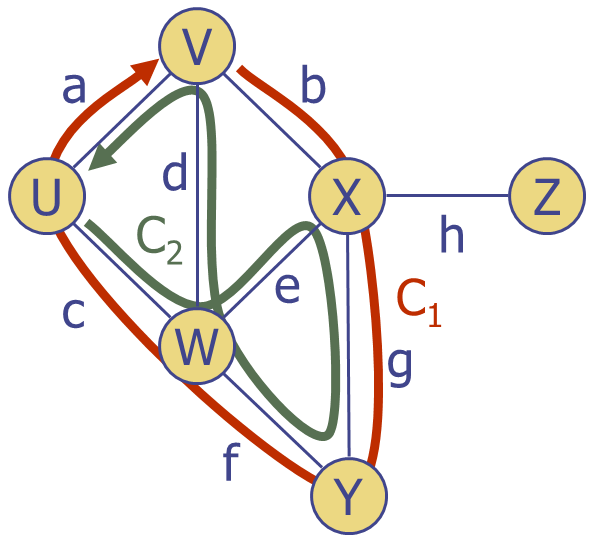
\includegraphics[width=4.5cm]{asp-14-pic06.png}
      \end{center}
    \end{column}
  \end{columns}
\end{frame}

\begin{frame}[fragile]
  \frametitle{Osobine}
  \begin{columns}
    \begin{column}[t]{7.5cm}
      \begin{itemize}
        \item suma stepena čvorova
        $$\sum_{v}deg(v)=2m$$ 
        \item u neusmerenom grafu bez petlji i 
        \begin{itemize}
          \item s vi čvorovi i grane su različiti
        \end{itemize}
        \item primeri
        \begin{itemize}
          \item $C_{1}=(V,b,X,g,Y,f,W,c,U,a,V)$ je prosta
          \item $C_{2}=(U,c,W,e,X,g,Y,f,W,d,V,a,U)$ nije prosta
        \end{itemize}
      \end{itemize}
    \end{column}
    \begin{column}[t]{4.5cm}
      \begin{center}
        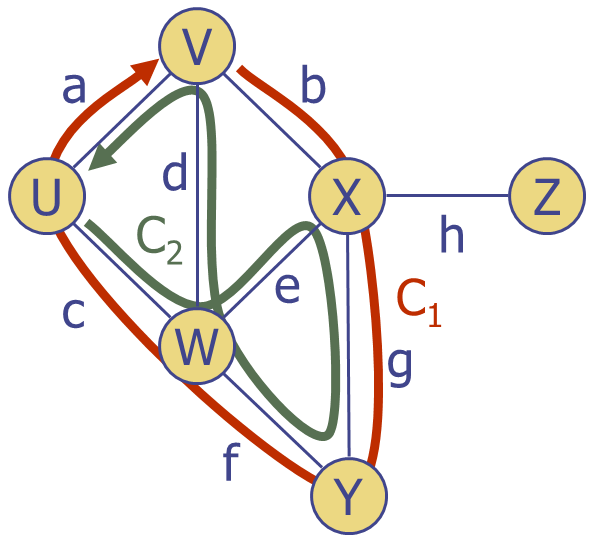
\includegraphics[width=4.5cm]{asp-14-pic06.png}
      \end{center}
    \end{column}
  \end{columns}
\end{frame}

\end{document}
